\documentclass[11pt,aspectratio=169,hyperref={colorlinks}]{beamer}

\usetheme{Singapore}

\usecolortheme[snowy]{owl}

\usepackage[utf8]{inputenc}
\usepackage[T1]{fontenc}
\usepackage[american]{babel}
\usepackage{graphicx}
\usepackage{hyperref}
\hypersetup{
    colorlinks=true,
    urlcolor=[rgb]{0,0,0.61},
    linkcolor=[rgb]{0,0,0.61}}
\usepackage[natbib=true,style=authoryear,backend=bibtex,useprefix=true]{biblatex}
\usepackage{blindtext}

%-------------------------------------------------------------------------------

\usepackage{mathtools}
\usepackage{xcolor}
\usepackage{soul}
\newcommand{\mathcolorbox}[2]{\colorbox{#1}{$\displaystyle #2$}}

%-------------------------------------------------------------------------------

% OwlGreen - customized to make the header violet color
\definecolor{OwlGreen}{RGB}{ 51, 0, 102}

%-------------------------------------------------------------------------------

\setbeamertemplate{bibliography item}{}
\renewcommand*{\bibfont}{\scriptsize}
\addbibresource{main.bib}

\setbeamerfont{caption}{size=\footnotesize}
\setbeamertemplate{frametitle continuation}{}
\setcounter{tocdepth}{1}

%-------------------------------------------------------------------------------

\usenavigationsymbolstemplate{}
\setbeamertemplate{footline}{%
    \raisebox{5pt}{\makebox{\hfill\makebox[20pt]{\color{gray}
          \scriptsize\insertframenumber}}}\hspace*{5pt}}

\renewcommand*{\thefootnote}{\fnsymbol{footnote}}

%-------------------------------------------------------------------------------

\author{Patrick Hall}
\title{Responsible Machine Learning\footnote{\tiny{This material is shared under a \href{https://creativecommons.org/licenses/by/4.0/deed.ast}{CC By 4.0 license} which allows for editing and redistribution, even for commercial purposes. However, any derivative work should attribute the author.}}}
\subtitle{Lecture 1: Interpretable Machine Learning Models}
\institute{The George Washington University}
\date{\today}

%-------------------------------------------------------------------------------

\begin{document}
	
	\maketitle
	
	\begin{frame}
	
		\frametitle{Contents}
		
		\tableofcontents{}
		
	\end{frame}
	

%-------------------------------------------------------------------------------
	\section{Class Overview}
%-------------------------------------------------------------------------------	
	\subsection*{}
	
	\begin{frame}
	
		\frametitle{Grading and Policy}
			
		\begin{itemize}
			\item{Grading:}
				\begin{itemize}
					\item{$\frac{1}{3}$ Participation}
					\item{$\frac{1}{3}$ Project GitHub or Kaggle kernel}
                    \item{$\frac{1}{3}$ Public Kaggle leaderboard score}
				\end{itemize}
			\item{Project:}	
				\begin{itemize}
					\item{Kaggle competition using techniques from class}
					\item{Individual or group (no more than 4 members)}
					\item Select team members ASAP
				\end{itemize}
			\item \href{}{Syllabus}
			\item{Webex office hours: Thurs. 5-6 pm or by appointment}
			\item{Class resources: \url{https://jphall663.github.io/GWU_rml/}}	
		\end{itemize}		
			
	\end{frame}
	
	
	\begin{frame}
	
		\frametitle{Overview}
		
		\begin{itemize}
			\item{\textbf{Class 1}: Interpretable Models}
			\item{\textbf{Class 2}: Post-hoc Explanations}
			\item{\textbf{Class 3}: Fairness}
			\item{\textbf{Class 4}: Security}
			\item{\textbf{Class 5}: Model Debugging}
			\item{\textbf{Class 6}: Best Practices}
		\end{itemize}
			
					
	\end{frame}

%-------------------------------------------------------------------------------
	\section{Introduction}
%-------------------------------------------------------------------------------
	
		\subsection*{}
			
		\begin{frame}
		
			\frametitle{A Responsible Machine Learning Workflow\footnote{\href{https://www.mdpi.com/2078-2489/11/3/137/htm}{\textit{A Responsible Machine Learning Workflow}}}}
			
			\begin{figure}[htb]
				\begin{center}
					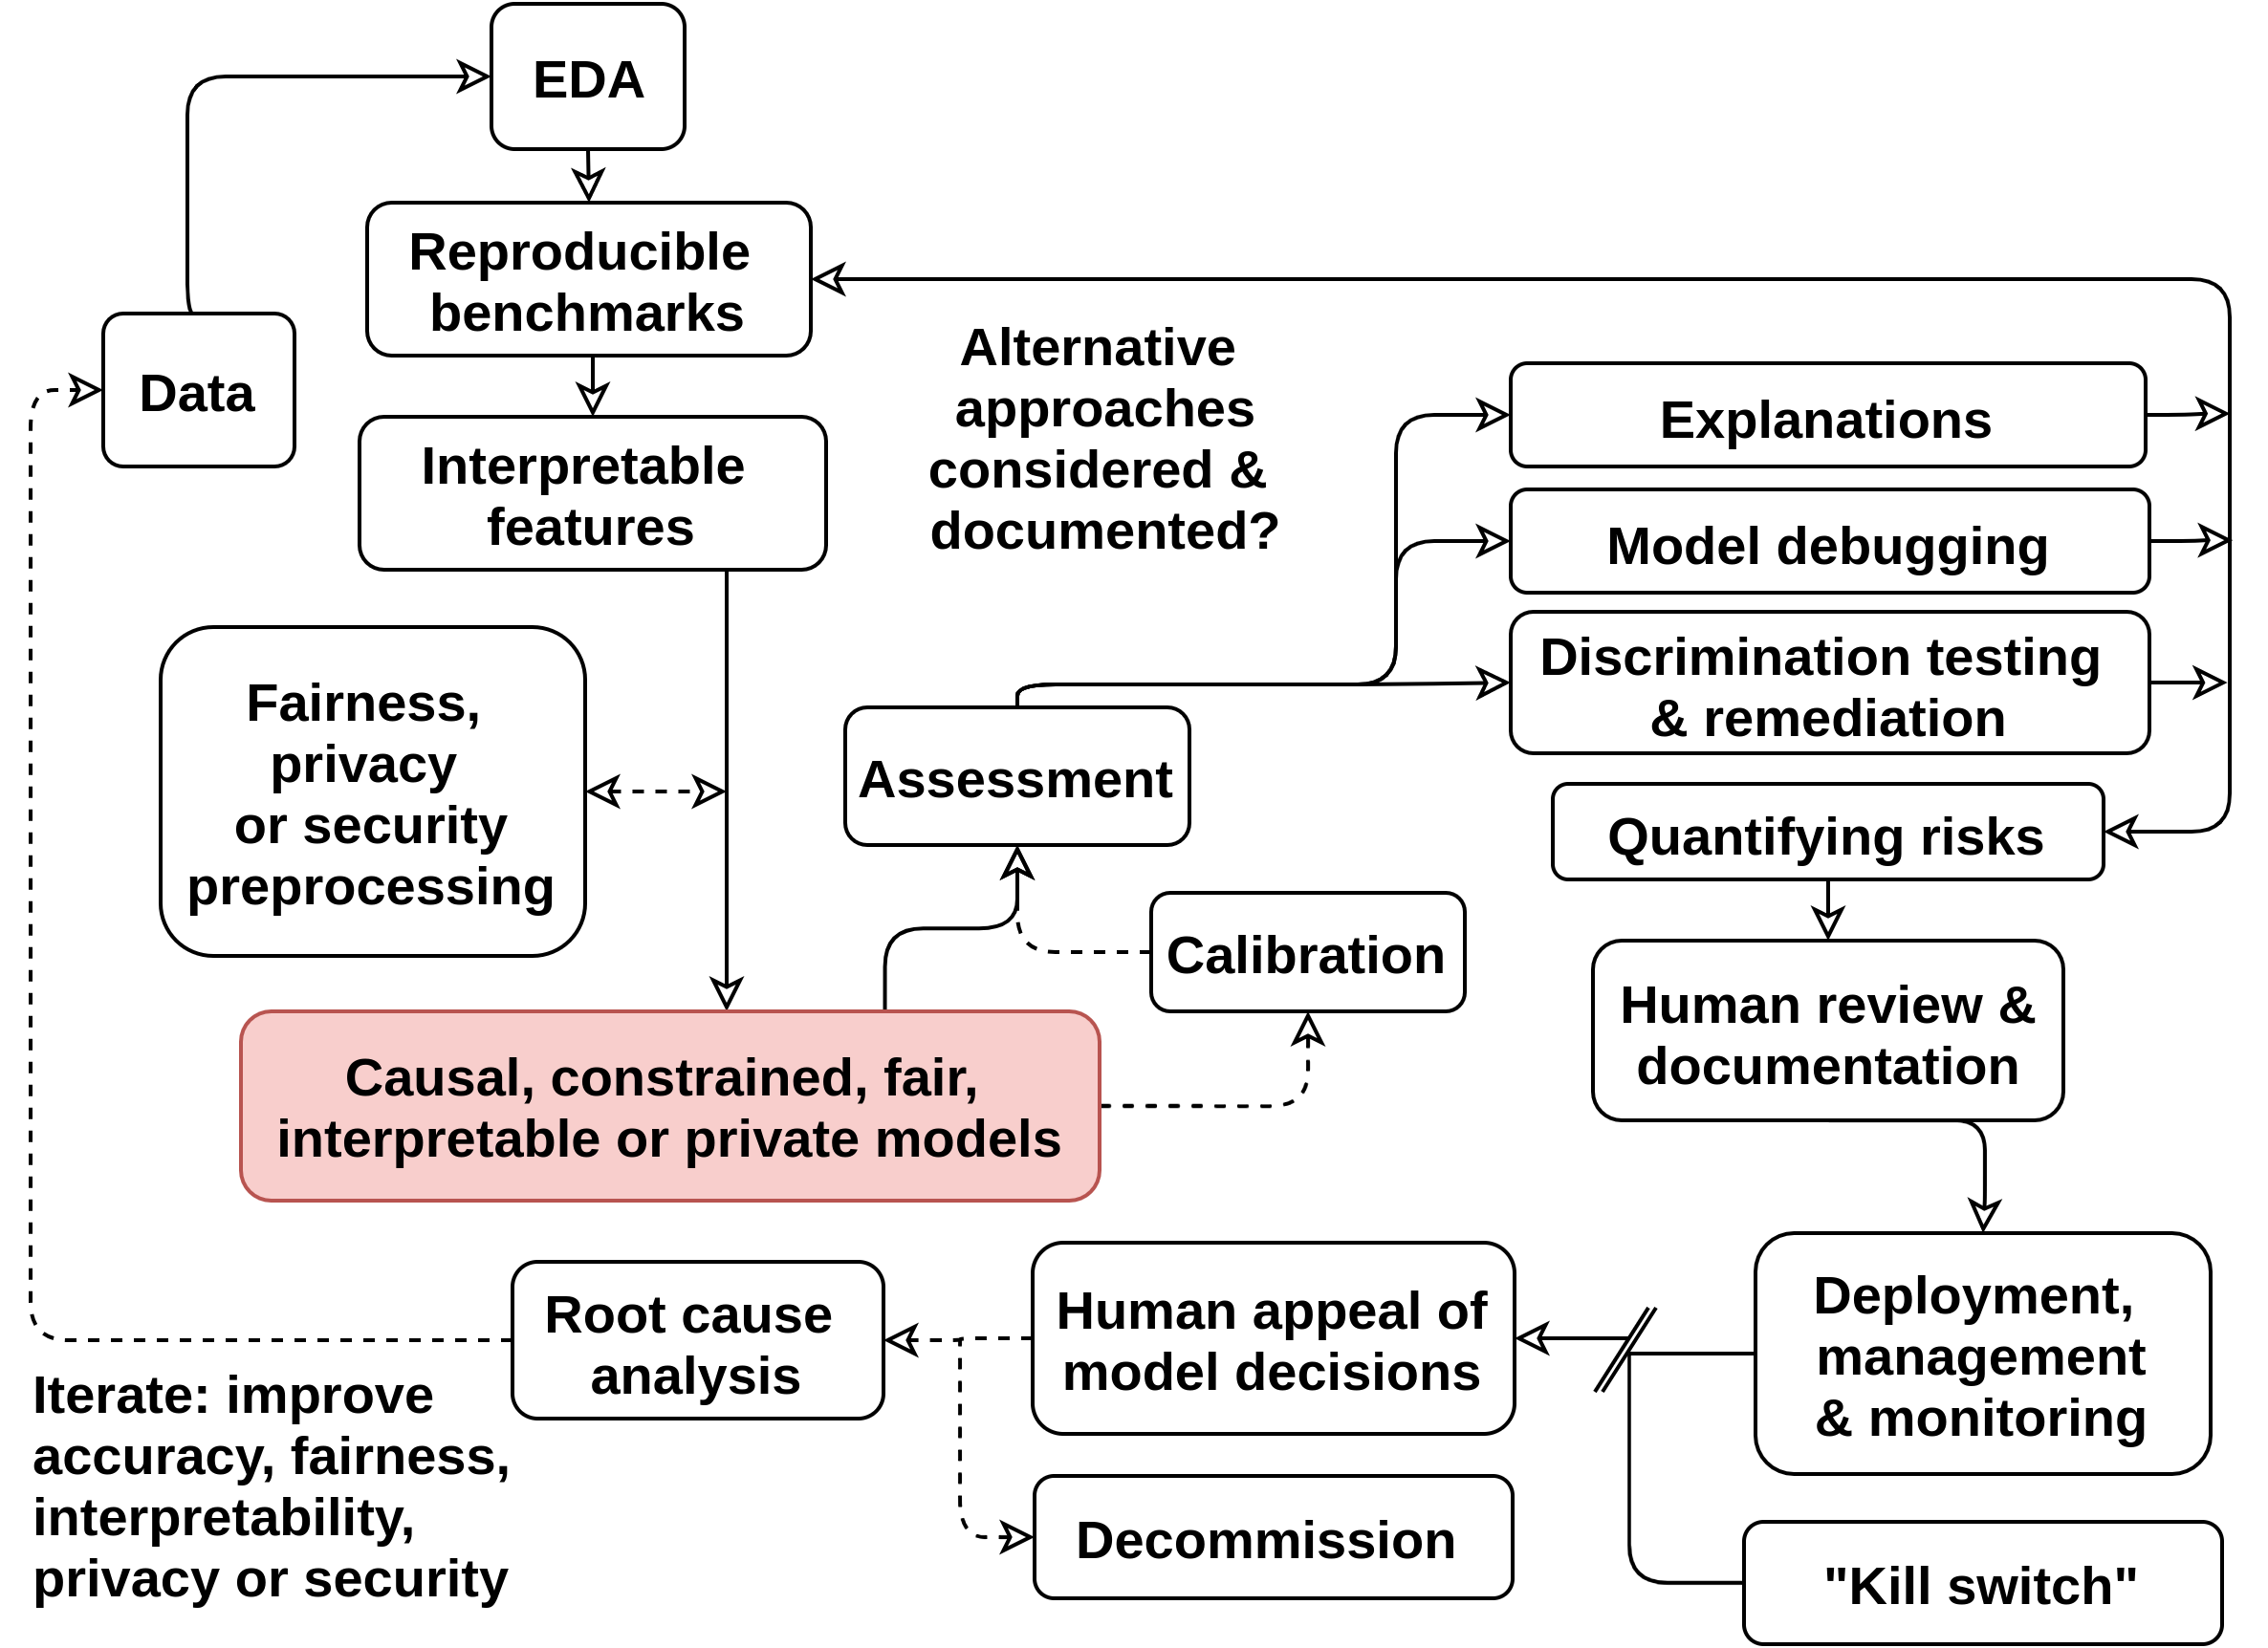
\includegraphics[height=150pt]{../img/rml_diagram_lec1_hilite.png}
					\label{fig:blueprint}
				\end{center}
			\end{figure}		
					
		\end{frame}					

		% fix/simplify
		\begin{frame}[allowframebreaks]
			
			\frametitle{Notation}
		
			\textbf{Spaces} 
 
			\begin{itemize}
				\item Input features come from the set $\mathcal{X}$ contained in a \textit{P}-dimensional input space, $\mathcal{X} \subset \mathbb{R}^P$.  An arbitrary, potentially unobserved, or future instance of $\mathcal{X}$ is denoted $\mathbf{x}$, $\mathbf{x} \in \mathcal{X}$.
				\item Labels corresponding to instances of $\mathcal{X}$ come from the set $\mathcal{Y}$.
				\item Learned output responses come from the set $\mathcal{\hat{Y}}$.
			\end{itemize}	
	
			\framebreak	
	
			\textbf{Datasets} 

			\begin{itemize}
				\item The input dataset $\mathbf{X}$ is composed of observed instances of the set $\mathcal{X}$ with a corresponding dataset of labels $\mathbf{Y}$, observed instances of the set $\mathcal{Y}$. 
				\item Each $i$-th observation of $\mathbf{X}$ is denoted as\\ $\mathbf{x}^{(i)} = $  
		$[x_0^{(i)}, x_1^{(i)}, \dots, x_{\textit{P}-1}^{(i)}]$, with corresponding $i$-th labels in $\mathbf{Y}, \mathbf{y}^{(i)}$, and corresponding predictions in $\mathbf{\hat{Y}}, \mathbf{\hat{y}}^{(i)}$.
				\item $\mathbf{X}$ and $\mathbf{Y}$ consist of $N$ tuples of observations:\\ $[(\mathbf{x}^{(0)},\mathbf{y}^{(0)}), (\mathbf{x}^{(1)},\mathbf{y}^{(1)}), \dots,(\mathbf{x}^{(N-1)},\mathbf{y}^{(N-1)})]$.
				\item Each $j$-th input column vector of $\mathbf{X}$ is denoted as $X_j = [x_{j}^{(0)}, x_{j}^{(1)}, \dots, x_{j}^{(N-1)}]^T$.
			\end{itemize}	 
	
			\framebreak
				
			\textbf{Models}

			\begin{itemize}
				\item A type of machine learning model $g$, selected from a hypothesis set $\mathcal{H}$, is trained to represent an unknown signal-generating function $f$ observed as  $\mathbf{X}$ with labels $\mathbf{Y}$ using a training algorithm $\mathcal{A}$: 
		$ \mathbf{X}, \mathbf{Y} \xrightarrow{\mathcal{A}} g$, such that $g \approx f$.
				\item $g$ generates learned output responses on the input dataset $g(\mathbf{X}) = \mathbf{\hat{Y}}$, and on the general input space $g(\mathcal{X}) = \mathcal{\hat{Y}}$.
				\item The model to be explained, tested for discrimination, or debugged is denoted as $g$.
			\end{itemize}
		
		\end{frame}


		\begin{frame}
		
			\frametitle{Background}		
			
			We will frequently refer to following terms and definitions today: \\			
			
			\begin{itemize}
				\item{Pearson correlation}
					\begin{itemize}
						\item{Measurement of the linear relationship between two input $X_j$; values between -1 and +1, including 0.}
					\end{itemize}
				\item{Shapley value}
				\item{Partial dependence and individual conditional expectation (ICE)}
				\item{Gradient boosting machine (GBM)}
			\end{itemize}			
		
		\end{frame}
		
		\begin{frame}
		
			\frametitle{Shapley Value}	
			
			Shapley explanations, including TreeSHAP and even certain implementations of LIME, are a class of additive, locally accurate feature contribution measures with long-standing theoretical support (\cite{shapley}). 

			\vspace{8pt}
			
			For some observation $\mathbf{x} \in \mathcal{X}$, Shapley explanations take the form:
			
			\begin{equation}
				\label{eq:shap_contrib}
				\begin{aligned}
					\phi_{j} = \underbrace{\sum_{S \subseteq \mathcal{P} \setminus \{j\}}\frac{|S|!(\mathcal{P} -|S| -1)!}{\mathcal{P}!}}_\text{weighted average over all subsets}\underbrace{(S \cup \{j\}) - g_x(S)]}_{g\text{ "without" }x_j}
				\end{aligned}
			\end{equation}
			
			\begin{equation}
				\label{eq:shap_additive}
				\begin{aligned}
					g(\mathbf{x}) = \phi_0 + \sum_{j=0}^{j=\mathcal{P} - 1} \phi_j \mathbf{z}_j
				\end{aligned}
			\end{equation}
			
		\end{frame}
		
		\begin{frame}
		
			\frametitle{Partial Dependence and ICE}			
			
			\begin{itemize}
			\item{Partial dependence (PD) plots are a widely-used method for describing the average predictions of a complex model across some partition of dataset for some interesting input feature (cite this - Friedman, Hastie, and Tibshirani, 2001)}
			\item{Individual conditional expectation (ICE) plots are a newer method that describes the local behavior of a complex model for a single input feature for each instances.  PD and ICE can be combined in the same plot to compensate for known weaknesses of partial dependence, to identify the interactions of the prediction model, and to create a holistic portrait of the predictions of a complex model for some input feature (cite)}
			\item{In simplier terms, the "PD plot is the average of all the ICE plot lines"}
			\end{itemize} 			
					
		\end{frame}		
		
		\begin{frame}
		
			\frametitle{GBM and Monotonic GBM}			
				  			
			\begin{itemize}
			\item{Gradient Boosting Machine (GBM)is a type of ensemble decision tree model (sequential) that is fitted by minimizing a loss function averaged over a training data}
			\item{The MGBMs constrain typical GBM training to consider only tree splits that obey user-defined positive and negative monotonicity constraints, with respect to each input feature and a target feature, independently}
			\end{itemize}
			
		\end{frame}	
				
%-------------------------------------------------------------------------------
	\section{Penalized GLM}
%-------------------------------------------------------------------------------
	
		\subsection*{}
	
		\begin{frame}[allowframebreaks]
		
			\frametitle{Anatomy of Elastic Net Regression: L1 and L2 Penalty}			
		Iteratively Resweighted Least Square method with generalized Ridge (L2) and LASSOS (L1) penalty terms: 
			
			\begin{equation}
				\label{eq:Elastic_Net}
				\begin{aligned}
				\tilde{\beta}= \underset{\beta}{min}\Big\{ \mathcolorbox{red}{ \underbrace{\sum_{i=1}^{N}(y_i-\beta_0-\sum_{j=1}^{p} x_{ij} \beta_j)^2}_\text{1}} + \mathcolorbox{red}{\underbrace{\lambda}_\text{2}} \sum_{j=1}^{p} ( \mathcolorbox{red}{\underbrace{\alpha}_\text{3}} \mathcolorbox{red}{\underbrace{\beta_j^2}_\text{4}} + (1-\mathcolorbox{red}{\underbrace{\alpha}_\text{3}}) \mathcolorbox{red}{\underbrace{|\beta_j|}_\text{5}}) \Big\}
				\end{aligned}
			\end{equation}		
			
			\begin{itemize}
			\scriptsize{
				\item{1: Least square minimization}
				\item{2: Controls magnitude of penalties}
				\item{3: Tunes balane between L1 and L2}
				\item{4: L2/Ridge penalty term}
				\item{5: L1/LASSO penalty term}}
			\end{itemize}
						
			\framebreak
			
			\textbf{Graphical Illustration of Shrinkage/Regularization Method:} 
			
			\begin{figure}[htb]
				\begin{center}
					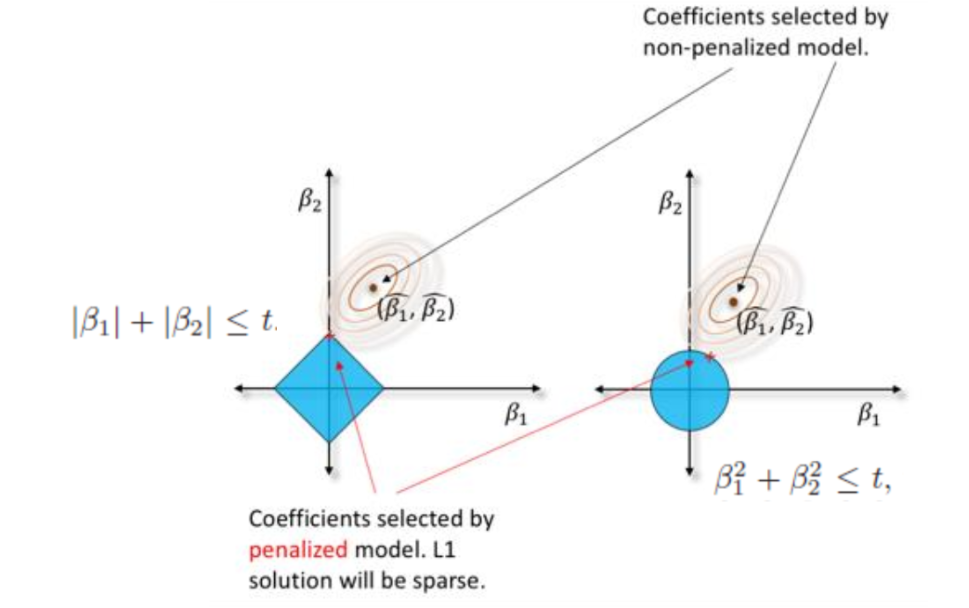
\includegraphics[height=150pt]{../img/L1L2_penalty_diagram.PNG}
					\label{fig:L1 and L2 Penalty Illustration}
				\end{center}
			\end{figure}
								
		\end{frame}				
		
%-------------------------------------------------------------------------------
	\section{Monotonic GBM}
%-------------------------------------------------------------------------------

	\subsection*{}
	
	\begin{frame}
	
		\frametitle{Monotonic GBM: Shapley Value}
		
		\textbf{MGBM and Shapley Value - insert content heres}
		
	\end{frame}


%-------------------------------------------------------------------------------
	\section{A Burgeoning Ecosystem}
%--------------------------------------------------------------------------
			
		\subsection*{}
		
		\begin{frame}
		
			\frametitle{Other Methods}		
			
			\begin{itemize}
				\item{GA2M/EBM}
				\item{XNN}
				\item{Scalable Bayesian Rulest List(C. Rudin)}
				\item{CORELS(C. Rudin)}
			\end{itemize}
		
		\end{frame}
		
		
%-------------------------------------------------------------------------------
%	References
%-------------------------------------------------------------------------------

	\begin{frame}[t, allowframebreaks]
	
		\frametitle{References}	
		
			\textbf{Link 1:}\\
			\small{\url{https://github.com/jphall663/}}
			
			\vspace{10pt}
			
			\textbf{Link 2:}\\
			\small{\url{https://www.h2o.ai}}
			
		\framebreak		
		
		\printbibliography
		
	\end{frame}

\end{document}
